\cotefile{136}
\scanpage{80}
\margin{Faisceautisation du topos De Rham}
1. Soit $X$ un topos, et
\[
\mathbb{Z}\xrightarrow{u}\Phi
\]
une immersion de $\mathbb{Z}$ dans un faisceau $\Phi$, tel que

a) $\operatorname{Coker}\Phi$ est $\mathbb{Z}$-plat

b) Pour tout $i>0$, $\Lambda_{\mathbb{Z}}^i\Phi$ et $\Gamma_{\mathbb{Z}}^i\Phi$ sont flasques, et le restent par tensorisation avec tout faisceau abélien.

En particulier, on en conclut \inserted{\deleted{par \unsure{récurrence} et dévissage}} que \deleted{\unsure{si}}

b') Si $i,j\geq 0$ et $i+j>0$, alors $\deleted{\Lambda}\Gamma_{\mathbb{Z}}^i\Phi\otimes\Lambda_{\mathbb{Z}}^j\Phi$ est flasque.

De b') on conclut \deleted{que}\inserted{(par récurrence et dévissage)}, posant
\[
\operatorname{Coker}i=\Psi
\]
\inserted{que} $\alpha$) les $\Gamma_{\mathbb{Z}}^i\Phi\otimes\Lambda_{\mathbb{Z}}^j\Psi$ sont flasques pour $i>0$. \unsure{$\vert$|1}

De $\unsure{\alpha|a|\text{ceci}}$) on conclut\unsure{:}\deleted{\unsure{que}}

$\beta$) Posant $K_u^{\bullet\bullet}=\Gamma_{\mathbb{Z}}^*\Phi\otimes\Lambda_{\mathbb{Z}}^*\Psi$, avec l'op. diff. \deleted{\unsure{$\delta$}} $d$ compatible aux puissances divisées qui, sur $\deleted{\unsure{\Gamma^0\otimes\Lambda^j}}\Psi$ est nul et sur $\unsure{\overline{\Phi}|\Phi}$ est l'hom canonique $\Phi\longrightarrow\Psi$, et définissant
\[
\mathbb{Z}\{T\}\longrightarrow\mathscr{H}^{*0}(K_u^{**})
\]
par $T\longmapsto 1\in\mathbb{Z}=\operatorname{Ker}(\Phi\xrightarrow{d}\Psi)$, et prolongeant par la condition d'être compatible aux p. div, on trouve que $K_u^{\bullet\bullet}$ est une \uline{résolution} de $\mathbb{Z}\{T\}$.

Utilisant encore a), \inserted{et b),} on trouve

$\gamma$) Pour tout faisceau d'anneaux comm. $k$ sur $X$, $K_{u,k}^{\bullet\bullet}\simeq K_u^{\bullet\bullet}\otimes k\simeq\Gamma_k^*\Phi_k\otimes\Lambda_k^*\Psi_k$ est une résolution de $k\{T\}\simeq\mathscr{H}^{\bullet 0}(K_{u,k}^{\bullet\bullet})$, et les $\Gamma_k^i\Phi_k\otimes\Lambda_k^j\Psi_k$ sont flasques pour $i>0$.
% archive sheet number: 79
\scanpage{81}
On va graduer $K_{u,k}^{\bullet\bullet}$ par a) le degré extérieur venant de $\Lambda_k^*\Psi_k$ ($\deg_{\mathrm{ext}}\Gamma^i\otimes\Lambda^j=j$) et b) le \uline{degré total} $i+j$. Ainsi $d$ augmente le degré extérieur par $1$, et invarie le degré total \deleted{\unsure{Kde}} (le degré complémentaire est $\deg_{\mathrm{comp}}\Gamma^i\otimes\Lambda^j=i$, il est diminué de $1$ par $d$.) Muni du degré total (ou complémentaire) $K_{u\,k}^{\bullet\bullet}$ est une Algèbre graduée sur l'Anneau gradué $k\{T\}$.

Conséquence (de $\gamma$ \unsure{disons de suite})

\uline{Théorème} Soit $K^{\bullet\bullet}(X,u,k)=\Gamma(X,K_{u,k}^{\bullet\bullet})$.

Alors on a un hom can (du fait que $K_{u\,k}^{\bullet\bullet}$ \deleted{\unsure{$K$}} est une résolution de $k\{T\}$)
\[
\begin{aligned}
H^{**}\deleted{\unsure{K}}(X,u,k)&\overset{\mathrm{dfn}}{=}H^{**}(K^{\bullet\bullet}(X,u,k))\\
&\longrightarrow H^{**}(X,k\{T\})\\
&\simeq H^*(X,k)\otimes_{\mathbb Z}\mathbb Z\{T\}
\end{aligned}
\]
et ceci est un isomorphisme pour les bidegrés $(i,j)$ tels que $\deleted{\unsure{i\leq j}}j\leq i$, tandis que $H^{i,j}(X,u,k)=0$ (et pour cause) pour $j>i$.

\figure{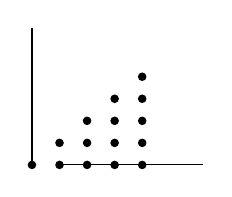
\begin{tikzpicture}[x=0.35cm,y=0.28cm]
\draw (0,6.2) -- (0,0); \draw (1,0) -- (6.2,0);
\foreach \x/\y in {0/0,1/0,1/1,2/0,2/1,2/2,3/0,3/1,3/2,3/3,4/0,4/1,4/2,4/3,4/4} {\fill (\x,\y) circle (1.55pt);}
\end{tikzpicture}}

\uline{Corollaire plus général.} Soit $f:X\unsure{\mathord{-}|\to}Y$ un morphisme de topos. Alors
\[
f_*K_{u,k}^{\bullet\bullet}\longrightarrow\mathbb R f_*(k\{T\})\simeq\mathbb R f_*(k)\otimes_{\mathbb Z}\mathbb Z\{\unsure{R|T}\}
\]
% archive sheet number: 80
\scanpage{82}
est un isomorphisme \inserted{en cohomologie} en bidegré $(i,j)$ avec $j\leq i$, tandis que la \unsure{coh.|ch.} du premier \unsure{mb} est nul pour $j>i$.

On peut l'exprimer comme un isomorphisme du $1^{\mathrm{er}}$ mb avec un certain tronqué du second....

\uline{Fonctorialités} a) en $k$, clair

b) \uline{En $u$}\deleted{\unsure{$\Phi$}} Soit
\[
u':\mathbb Z\longrightarrow\Phi'
\]
une deuxième immersion, S'il existe un hom $\lambda:\Phi\longrightarrow\Phi'$ rendant comm.
\diagram{\begin{tikzcd}[ampersand replacement=\&,column sep=small]
\& \mathbb Z\arrow[dl,"u"']\arrow[dr,"u'"] \& \& \\
\Phi\arrow[rr,"\lambda"] \& \& \Phi' \& \text{i.e.}\quad\lambda u=u'
\end{tikzcd}}
\deleted{\unsure{Eh}}On en conclut $\widetilde\lambda:K_u^{\bullet\bullet}\unsure{\mathord{-}|\to}K_{u'}^{\bullet\bullet}$ et $\widetilde\lambda_k:K_{u,k}^{\bullet\bullet}\longrightarrow K_{u',k}^{\bullet\bullet}$, compatible avec \unsure{ttes} les structures, qui est un isom. dans telle catégorie dérivée, et le reste après application de $\Gamma(X,-)$ ou de $f_*$.

Supposons qu'on ait un autre, soit $\mu$, tel que
\[
\mu u=u'
\]
alors, posant $\mu=\lambda+\Theta$,

on trouve $\Theta u=0$
% archive sheet number: 81
\scanpage{83}
$K^{\bullet\bullet}$ Algèbre de DR à p.d. élémentaire

a) Anneau bigradué \inserted{à bidegr. $\geq 0$}, \deleted{\unsure{comm.}} alterné pour \inserted{``deg. ext''}

b) \deleted{\unsure{Système}} Structure à p. d. sur l'idéal $\sum_{i+j>0}K^{ij}$

c) différentielle d'Anneau gradué (pour la grad ext) ne changeant pas le degré total, et comp. \unsure{avec|aux} p. d.

d) $d:K^{1,0}=\Phi\longrightarrow K^{11}\unsure{\equiv|=}\Psi$ est un épi.

e) Posant $k=K^{00}$, $K^{**}$ est l'algèbre \inserted{alternée} à p. d. libre engendrée par $\Phi$ et $\Psi$ i.e. $K^{**}\simeq\Gamma^*\Phi\otimes\Lambda^*\Psi$ [Il en résulte que $K^{ij}=0$ si $j>i$.]

f) \deleted{\unsure{$\Psi$ est $k$-plat|Mono-plat}} $\Phi$ et $\Psi$ sont $k$-plats (donc aussi $L=\operatorname{Ker}d=\mathscr H^{10}(K^{\bullet\bullet})$)

Il résulte déjà de ceci que
\[
H^{*i}(K^{\bullet\bullet})=
\begin{cases}
\Gamma^*L & \text{si }i=0\\
0 & \text{si }i>0
\end{cases}
\]
donc que $K^{\bullet\bullet}$ est une résolution de $\Gamma^*L$. On va supposer le plus souvent

g) $L$ est un $k$-Module \deleted{inversible}\inserted{loc. libre de rg} $1$.

(voire libre de rang $1$ et trivialisé ...)
% archive sheet number: 82
\scanpage{84}
% Typescript rotated 180 degrees in the scan.
% letterhead
UNIVERSITE DES SCIENCES ET TECHNIQUES\hfill MONTPELLIER, le 10 juillet 1975\\
DU LANGUEDOC\\
Mathématiques

\uline{JOURNEES MATHEMATIQUES S.M.F.}

"Formes quadratiques et questions connexes"

18 au 22 novembre 1975

(1ère annonce)

A l'heure actuelle, les conférenciers suivants ont accepté de participer à ces journées d'études :

H. GROSS, Mathematisches Institut der Universität Zurich

Formes quadratiques et sesquilinéaires dans les espaces de dimension infinie.

A. FROHLICH, University of London

Hermitian class group of integral group rings and arithmetic applications.

W. SCHARLAU, Mathematisches Institut der Universität Münster

Quadr\unsure{a|e}tic forms in additive categ\deleted{\unsure{n}}ories (titre provisoire)

A. GRAMAIN, Université de Tours

Titre non parvenu.

O. LABORDE, Université de MONTPELLIER

Classes caractéristiques d'un module quadratique en cohomologie étale.

Mme C. HØSTMAELINGEN, Université d'Oslo

Anneaux de Witt des anneaux de Prüfer.

A. MICALI et Ph REVOY, Université de M\unsure{on}tpellier

Sur l'existence de produits vectoriels et variétés de Stiefel algébriques.

Pour tout renseignement concernant ce colloque, vous êtes priés de vous adresser à :

Mme P. ARNAUD\\
Secrétaire de l'U.E.\unsure{R}. de Mathématiques\\
Université des Sciences et Techniques du Languedoc\\
Place Eugène Bataillon\\
34060 MONTPELLIER CEDEX

\begin{center}\rule{2.3cm}{0.4pt}\end{center}
% archive sheet number: 83
\scanpage{85}
\deleted{\unsure{Soient} $K^{\bullet\bullet}$ et $K^\bullet$}

Finalement, la donnée de $K^{\bullet\bullet}$ équivaut à celle de

$\alpha$) $k$, Anneau comm sur $X$

$\beta$) $L$, $k$-Module plat (voire inversible voire $k$ lui-$=$ ...)

$\gamma$) Une immersion de $L$ dans un $k$-module $\Phi$, $u:L\unsure{\mathord{-}|\to}\Phi$.

Soit de $=$ $K^{\prime\bullet\bullet}$ défini par $(k',L',\Phi',u')$. \deleted{\unsure{on}} La donnée d'un hom \inserted{$\lambda$} de $K^{\bullet\bullet}$ dans $K^{\prime\bullet\bullet}$, compatible avec \unsure{ttes} les structures, équivaut à la donnée d'un syst. d'hom
\[
\begin{aligned}
k&\xrightarrow{\deleted{\unsure{\lambda_0}}\lambda_0}k' &&\text{hom d'Anneaux}\\
&\deleted{\unsure{L\xrightarrow{\lambda_L}L'|K^{\bullet\bullet}\to K^{\prime\bullet\bullet}}}\\
\Phi&\xrightarrow{\lambda_\Phi}\Phi' &&\deleted{\unsure{\text{un}}}\inserted{\text{hom }\lambda_0\text{-}\tfrac12\text{ linéaire}}
\end{aligned}
\]
avec \deleted{\unsure{compatible dans}}\inserted{$\lambda_\Phi(u(L))\subset u'(L')$, donc $\lambda_\Phi$} induit un hom (évidemment $\lambda_0$-$\frac12$\unsure{lin-})
\diagram{\begin{tikzcd}[ampersand replacement=\&,row sep=small]
\deleted{L}\arrow[r,"{\deleted{\unsure{\lambda|\lambda_L}}}",dash]\arrow[d] \& \deleted{L'}\arrow[d]\\
% Oblique cancellation strokes cross the square.
\deleted{\Phi}\arrow[r,dash]\arrow[ur,dash,shift left=0.8ex]\arrow[ur,dash,shift right=0.8ex] \& \deleted{\Phi'}
\end{tikzcd}}
\[
L\xrightarrow{\lambda_L}L'
\]
Dans le cas $L\simeq k$, $L'\simeq k'$ donnés, on peut oublier $L,L'$ et retenir $\Phi,\Phi'$ avec sections marquées, et la condition sur $\lambda_\Phi$
% archive sheet number: 84
\scanpage{86}
% letterhead
UNIVERSITE DES SCIENCES \hfill Montpellier, le 17 Juillet 1975\\
ET TECHNIQUES DU LANGUEDOC\\
\texttt{-{}-{}-{}-{}-{}-{}-{}-{}-{}-}\\
Service de la Scolarité\\
AMC/GJ

\uline{Diffusion} : Liste H\\
N°4617

AVIS DE SOUTENANCE\\
D'UNE THESE DE DOCTORAT D'ETAT

\begin{center}\rule{2cm}{0.4pt}\end{center}

% printed form
\uline{Nom et prénom du candidat} : FOLLET Michel

\uline{Titre de la Thèse} : Etude physicochimique de la réactivité du cycle triazine : Synthèse et analyse spectrale de dérivés bicycliques.

\uline{Date, heure et lieu de soutenance prévus} :\\
8 Septembre 1975 à 17 Heures,\\
Salle de cours n° 9.

\uline{Nom du Directeur de thèse} : Professeur JACQUIER.

\uline{Désignation du laboratoire où la thèse est préparée} : Laboratoire de Synthèse et d'Etude Physicochimique d'Hétérocycles Azotés.

\uline{Résumé de la thèse} : Ce travail porte sur la série de la triazine - 1,2,4 , plus particulièrement sur les dérivés de l'acide thioxo-3 oxo-5 tétrahydro-2,3,4,5 triazine carboxylique -6. Différentes méthodes de synthèse de triazolo-triazines et triazolyl - triazines sont données. L'analyse spectrale de ces composés est faite par UV, RMN et spectrométrie de masse.

\uline{Durée approximative des recherches ayant abouti à la thèse} : 4 ans.

\uline{Noms des rapporteurs} :

JACQUIER R., Professeur, Chimie organique, U.S.T.L.\\
GRANGER R., Professeur, Chimie organique; Université MONTPELLIER I.\\
VIALLEFONT Ph. Professeur, Chimie organique, U.S.T.L.

\uline{Composition du jury} :

JACQUIER R., Professeur, Chimie organique, U.S.T.L. (Président)

GRANGER R., Professeur, Chimie organique, Université MONTPELLIER I (Membre extérieur choisi en raison de sa compétence scientifique)

DESCHAMPS J. Professeur, Chimie-physique, Faculté de Pau et des Pays de l'Adour (Membre étranger à la spécialité du candidat)

VIALLEFONT Ph. Professeur, Chimie organique, U.S.T.L.

DAUNIS J., Chargé de Recherche CNRS, Chimie organique, U.S.T.L.

LE SECRETAIRE GENERAL\\
\handwritten{\unsure{E S}}\\
\uline{E. SIAU}

% address label, lower left
MR LE PROFESSEUR GROTHENDIECK A.\\
MATHEMATIQUES \hfill 5-856
% archive sheet number: 85
\scanpage{87}
devient alors de transformer section marquée en section marquée.

Supposons que nous ayons deux hom $\lambda,\mu$, correspondant à un \uuline{$=$} \unsure{homom.}
\[
k\xrightarrow{\lambda_0=\mu_0}k'
\]
et deux hom
\diagram{\begin{tikzcd}[ampersand replacement=\&]
\Phi\arrow[r,shift left=.7ex,"{\lambda_\Phi,\mu_\Phi}"]\arrow[r,shift right=.7ex] \& \Phi'
\end{tikzcd}}
(ayant $=$ effet sur la section marquée)

Que peut-on dire des hom $\lambda,\mu$ de $K^{\bullet\bullet}$ dans $K^{\prime\bullet\bullet}$ ?
% archive sheet number: 86
\scanpage{88}
% Typescript rotated 180 degrees in the scan.
% letterhead
U N I V E R S I T E \hfill Montpellier, le 16 Juillet 1975\\
DES SCIENCES ET TECHNIQUES\\
DU LANGUEDOC\\
\texttt{-{}-{}-{}-{}-{}-{}-{}-{}-{}-{}-{}-}

AMC/GJ\\
\uline{Diffusion} : Liste A\\
N°4549

\uline{AVIS DE SOUTENANCE D'UNE THESE DE DOCTEUR-INGENIEUR}

% printed form
\uline{Nom et prénom du candidat} : DASSOUKI Mouhiddine

\uline{Titre de la thèse} : Etude expérimentale et théorique d'une machine à courant continu à commutation par thyristors tournant avec l'induit.

\uline{Date, heure et lieu de soutenance prévus} :\\
29 Juillet 1975 à 10 Heures\\
Salle de cours n° 9.

\uline{Nom du Directeur de thèse} : R. JOUTY

\uline{Désignation du laboratoire où la thèse est préparée} : Laboratoire de Physique des Métaux.

\uline{Analyse de l'ouvrage} : Il est possible de remplacer le collecteur d'une machine à courant continu classique par une batterie de thyristors. Pour la commande de ces derniers, leurs gachettes sont reliées à un collecteur auxiliaire. L'étude de ce type nouveau de machine fait apparaître des similitudes, mais aussi de grandes différences avec la machine classique; notamment en ce qui concerne la commutation et la réaction d'induit, dont l'auteur donne une analyse très détaillée. L'étude expérimentale, faite sur un prototype obtenu par transformation d'une machine classique, est en bon accord avec la théorie, et fait apparaître des performances satisfaisantes.

\uline{Durée approximative des recherches ayant abouti à la thèse} : 2 ans.

\uline{Composition du jury proposé} :\\
Monsieur JOUTY R.\\
Monsieur GROUBERT E.\\
Monsieur TROMPETTE

LE SECRETAIRE GENERAL,\\
\handwritten{E S}\\
\uline{E. SIAU}
% archive sheet number: 87
\scanpage{89}
$X$, topos

$k$ Anneau sur $X$

$k\overset{u}{\lhook\joinrel\longrightarrow}\Phi$ mono dans $k$-Module, avec
\[
\left\{\begin{aligned}
&\text{\textcircled{a}}\quad \deleted{\unsure{\Phi}}\Psi=\operatorname{Coker}u\quad k\text{-plat}\\
&\text{\textcircled{b}}\quad\forall\, k\text{-modules }M,N,\ \text{et }i\unsure{\geq|>}0\\
&\hspace{1em}\Gamma^i(M\otimes_k\Phi)\otimes N\unsure{T|]}\ \text{est flasque}
\end{aligned}\right.
\]

\uline{Lemme} $\forall$ $k$-module $\unsure{S|B|N}$, $\exists$ \deleted{\unsure{hom|homom.}} $S\xrightarrow{u_S}\widetilde N$, qui \textcircled{a'} est un $k$-mono \textquotedblleft universel'' (reste mono par tensorisation) \deleted{\unsure{tel que}} $S$ plat $\Rightarrow\operatorname{Coker}u_{\unsure{N|S}}$ plat, et \textcircled{b'} $\forall i>0$, et $k$ modules $\deleted{N}P,M$ $\Gamma_k^i(\widetilde N\otimes_k P)\otimes_k M$ flasque

On prend $\widetilde N=\Phi\otimes_k S$, $u_S=u\otimes\mathrm{id}_S$, alors a') résulte de a), et b') de b)

$\mathscr{DR}^{**}_{pd}(\deleted{\unsure{X,}}k,u)=\Gamma^*(\Psi)\otimes_k\Lambda^*\Psi$ Anneau bigradué (degré compl + degr. ext = degré total) \inserted{alterné (pour degr. ext)}, différentiel à p.d. (sur idéal des bidegrés $>0$ \unsure{...|?}) \unsure{une|...|---} résolution de $k\{T\}$. (où $\deg\mathrm{ext}\,T=0$, $\deg\mathrm{tot}\,T=1$)
\[
\mathrm{DR}_{pd}^{**}(k,u)=\Gamma(X,\mathscr{DR}_{pd}^{**}(k,u)).
\]

Soit $\mathbb{DR}^{**}$ la cat \inserted{dérivée} des anneaux bigradués (à degr $\geq 0$) alternés diff à p.d. \deleted{\unsure{un}}\inserted{avec \deleted{\unsure{unité}}\inserted{élément} \unsure{marqué pur} bidegré $(1,0)$} On va définir un \unsure{syst.|système} transitif d'isom. dans $\mathbb{DR}^{**}$ entre les $\mathrm{DR}_{pd}^{**}(k,u)$, pour $k$ fixé et $u$ variable

Notons que si on a
\diagram{\begin{tikzcd}[ampersand replacement=\&,row sep=small]
\& \Phi\arrow[dd,"\lambda"]\\
k\arrow[ur,"u"]\arrow[dr,"u'"'] \&\\
\& \Phi'
\end{tikzcd}}
d'où $\lambda^{**}:\mathrm{DR}_{pd}^{**}(k,u)\unsure{\mathord{-}|\to}\mathrm{DR}_{pd}^{**}(k,u')$, alors $\lambda^{**}$ est un iso. dans $\mathbb{DR}^{**}$

\diagram{\begin{tikzcd}[ampersand replacement=\&,column sep=small,row sep=small]
\&\Phi'\arrow[dr,hook]\&\&\\
k\arrow[ur,hook,"u"]\arrow[dr,hook,"u'"']\&\& S\arrow[r,hook,"\text{donné par lemme}"]\arrow[d,phantom,"\Vert" description]\&N\\
\&\Phi\arrow[ur,hook]\&\Phi\amalg_k\Phi'\&
\end{tikzcd}}
d'où
\diagram{\begin{tikzcd}[ampersand replacement=\&,row sep=small]
\mathrm{DR}(u)\arrow[dr,"\sim"]\&\\
\&\mathrm{DR}(N)\\
\mathrm{DR}(u')\arrow[ur,"\sim"']\&
\end{tikzcd}}
d'où $\mathrm{DR}(u)\simeq\mathrm{DR}(u')$ dans $\mathbb{DR}^{**}$

indépendance du choix de $S\hookrightarrow N$ avec $N$ comme dans le lemme
\diagram{\begin{tikzcd}[ampersand replacement=\&,column sep=small,row sep=small]
\&\&N\arrow[dr,hook]\&\&\\
k\arrow[r,phantom,"{-}" description]\&S\arrow[ur,hook]\arrow[dr,hook]\&\&\unsure{T''|T}\arrow[r,hook,"\text{donné par lemme}"]\arrow[d,phantom,"\Vert" description]\&N''\\
\&\&N'\arrow[ur,hook]\&N\amalg_S N'\&
\end{tikzcd}}
d'où
\diagram{\begin{tikzcd}[ampersand replacement=\&,column sep=small,row sep=small]
\mathrm{DR}(u)\arrow[dr]\&\&\mathrm{DR}(N)\arrow[dr,"\sim"]\&\&\\
\&\mathrm{DR}(S)\arrow[ur]\arrow[dr]\&\&\mathrm{DR}\,N''\&\unsure{\mathord{\sim}}\\
\mathrm{DR}(u')\arrow[ur]\&\&\mathrm{DR}(N')\arrow[ur,"\sim"']\&\&
\end{tikzcd}}

Transitivité évidente par diagramme
% archive sheet number: 88
\scanpage{90}
\mspage{- 175 -}
\hfill IX

\[
0\longrightarrow R^f/R^t\longrightarrow E/E^t\longrightarrow B\longrightarrow 0\quad . \tag*{(13.3.15)}
\]

On notera que
\[
R^f/R^t=(R_{\unsure{o|0}}/R_o^t)_S \tag*{(13.3.16)}
\]
est un groupe analytique constant sur $S$. Il résulte donc de 13.1.5 que $B$ est un groupe abéloide sur $S$ au voisinage de $s$ si et seulement si sa fibre en $s$
\[
B_o=A_o/T_o
\]
est un groupe analytique abéloide, de sorte que $A_o$ apparaît alors comme une extension d'un tel groupe $B_o$ par un tore $T_o$. \uline{Toute façon d'écrire} $A_o$ \uline{sous forme d'une extension d'un groupe abéloide par un tore complexe} (*) \uline{donne donc naissance sur} $A$ , \uline{au voisinage de} $s$, \uline{à une unique structure d'extension} (13.3.13) \uline{d'un groupe abéloide} $B$ \uline{par un tore} $T$, \uline{induisant la structure d'extension donnée en} $s$.

13.4. \uline{Interprétation en termes de} "\uline{structures de Hodge mixtes}" \uline{de DELIGNE}.

Reprenons d'abord le dictionnaire 13.1.4, que nous allons reformuler d'une façon légèrement différente,mieux adaptée à l'introduction des "structures de Hodge" pertinentes à la situation. Pour ceci, soit $\mathbb R$ le faisceau des sections de $R$ sur $S$, et introduisons le $\underline{O}_S$-Module
\[
\mathscr E(A)=\mathscr E=\underline R\otimes_{\mathbb Z}\underline O_S\quad , \tag*{(13.4.1)}
\]
qui est localement libre de type fini lorsque $R$ est localement constant. (NB Le faisceau $\mathscr E$ n'est pas nécessairement cohérent si $R$ n'est pas localement constant.) L'homomorphisme (13.1.3) $\underline R\longrightarrow\underline E$ définit alors

% Faint, partly covered numerals at lower strip. Attribution uncertain.
\margin{\unsure{493|1193} \illegible{1}}
% printed label at foot
493
% archive sheet number: 89
\scanpage{91}
\diagram{\begin{tikzcd}[ampersand replacement=\&,column sep=small,row sep=tiny]
\&\Phi\arrow[r,dash]\&N\arrow[dddr,dash]\&\\
\&\&\&\\
k\arrow[uur,"u"]\arrow[r,"u'"]\arrow[dr,dash,"{\deleted{\unsure{u'}}}"']\arrow[ddr,"u''"']\&\Phi'\arrow[uur,dash]\arrow[ddr,dash]\&\&\\
\&\deleted{\Phi'}\&\&N''\\
\&\Phi''\arrow[r,dash]\&N'\arrow[ur,dash]\&
\end{tikzcd}}
d'où
\diagram{\begin{tikzcd}[ampersand replacement=\&,row sep=small]
\&\Phi\arrow[dr]\&\\
k\arrow[ur]\arrow[r]\arrow[dr]\&\Phi'\arrow[r]\&N''\\
\&\Phi''\arrow[ur]\&
\end{tikzcd}}
\diagram{\begin{tikzcd}[ampersand replacement=\&,row sep=small]
\mathrm{DR}(\Phi)\arrow[dr,"\sim"]\&\\
\mathrm{DR}(\Phi')\arrow[r,"\sim"]\&\mathrm{DR}(N'')\\
\mathrm{DR}(\Phi'')\arrow[ur,"\sim"']\&
\end{tikzcd}}

Argument analogue pour $f_*(\mathscr{DR}^{**}_{pd}(k,u))$, si $f:X\unsure{\mathord{-}|\to}Y$ morphisme de topos.

\uline{Condition} de \uline{De Rham sur Anneau} $k$ : la condition d'existence d'un $u:k\mathord{-}\Phi$ tel que....

Si $k$ satisfait condition de De Rham, de $=$ \unsure{tte|tt} $k$-Algèbre. Donc le plus beau, c'est que $\mathbb Z_X$ y satisfasse ! C'est vrai pour

a) le topos \unsure{ss|SS} $\widehat{\Delta}$

b) le topos défini par un espace topologique paracompact.

\uline{Question} Est-ce vrai pour $\widehat{\Delta^\circ}$ (topos des ens. cosimpliciaux) ? \shortstack{\uuline{Non}\\[-0.7ex]\rule{1.9em}{0.4pt}}

Soit $A^{**}\in\operatorname{Ob}\mathbb{DR}^{**}_{pd}(X)$ une Algèbre bigraduée à degrés positifs, alternée pour le degré ext, diff. à p. div. ... Supposons que $A^{00}=k$ satisfasse la condition de De Rham, soit $u:k\longrightarrow\Phi$ d'où $\mathscr{DR}^{**}_{pd}(k,u)$. Considérons alors
\[
\overline{A^{**}}=\mathscr{DR}^{**}_{pd}(A^{**})\overset{\mathrm{dfn}}{=}\mathrm{DR}^{**}_{pd}(k)\deleted{\unsure{u,}}\otimes_{k\{T\}}A^{**},
\]
l'augmentation $k\{T\}\mathord{-}\mathrm{DR}_{pd}^{\unsure{*|**}}(\unsure{k,u|k})$ \inserted{(qui est un quasi-iso\unsure{.} \uline{universel})}, définit un hom
\[
A^{**}\longrightarrow\overline{A^{**}}
\]
qui est un quasi-iso. \deleted{\unsure{De plus}}\inserted{En effet}
% archive sheet number: 90
\scanpage{92}
\mspage{- 174 -}
\hfill IX

(13.3.9) correspond simplement à l'homomorphisme
\[
E^t/R_{\unsure{o|0}S}^t=E^t/R^t\longrightarrow E/R_{oS}=E/R^f
\]
induit par les inclusions
\[
E^t\hookrightarrow E,\quad R^t\hookrightarrow R^f\quad .
\]

Utilisant le fait que (13.3.9) induit une immersion sur les fibres en $s$, on en conclut que l'homomorphisme
\[
R_o/R_o^t\longrightarrow E_o/E_o^t=(E/E^t)_o
\]
est injectif, d'où il résulte aussitôt que
\[
R_o/R_o^t\longrightarrow(E/E^t)_{s'}
\]
est encore injectif pour $s'$ voisin de $s$, ce qui implique que, quitte à rapetisser $S$ autour de $s$, on peut supposer que (13.3.9) \uline{est une immersion fermée}.

Il s'impose alors d'introduire
\[
B=A^{\handwritten{\natural}}/T\simeq(E/E^t)/(R^f/R^t)\quad , \tag*{(13.3.12)}
\]
de sorte qu'on obtient sur $A^{\handwritten{\natural}}$ une structure d'extension
\[
0\longrightarrow T\longrightarrow A^{\handwritten{\natural}}\longrightarrow B\longrightarrow 0\quad , \tag*{(13.3.13)}
\]
$B$ étant un groupe analytique relatif sur $S$, lisse et séparé sur $S$ et à fibres connexes. Par construction même, on a donc
\[
\underline{\mathrm{Lie}}(B)\simeq\underline E/\underline E^t\quad , \tag*{(13.3.14)}
\]
et la suite exacte exponentielle pour $B$

% Faint, partly covered numerals at lower strip. Attribution uncertain.
\margin{\unsure{492|1192}}
% printed label at foot
492
% archive sheet number: 91
\scanpage{93}
% Blank face of perforated stationery. Faint reversed printing shows through at the left.
% archive sheet number: 92
\scanpage{94}
\deleted{(à p. div. -- sous} Cat. dér. des Alg. de De Rham spéciales

Structure De Rham (à p.d. -- sous-entendu)

Anneau bigradué [à degrés -- total et ext -- $\geq 0$] alterné pour degré ext
\[
 A^{ij}\ne 0\quad\deleted{\unsure{\Leftarrow|et}}\Rightarrow
 \deleted{\unsure{j}}0\leq j\leq i
\]
degré complémentaire $=\unsure{j|i}-j\geq 0$

différentiel [différentielle de bidegré $0,1$ ; c'est une diff. pour le degré ext \deleted{\unsure{$j$|:}}
\[
d(xy)=(dx)y+(-1)^{\deg.\mathrm{ext}\,x}x\,dy
\]
]

à p. div. sur l'idéal $\displaystyle\sum_{i+j>0} A^{ij}=A^+$ [p. div. \deleted{\illegible{1}} compatible aux 2 grad \deleted{\unsure{$d$}} $(\gamma^d:A^{ij}\longrightarrow A^{di,dj})$ et la différentielle $(d\,x^{(i)}=x^{(i-1)}dx)$]

\uline{élément marqué} $T\in Z^{10}(A^{**})\simeq H^{10}(A^{**})$

[Cohomologie $H^{*i}(A^{**})\simeq\unsure{\tau_i|\prod_i|[}h^i\otimes_k k\{T\}$, \deleted{\unsure{où|$0$}}] $k=A^{00}$

Structure de De Rham \uline{spéciale} :
\[
\left\{\begin{aligned}
k\{T\}&\xrightarrow{\sim}H^{*0}(A^{**})\\
H^{*i}(A^{**})&=0\\
\text{les } A^{ij}&\text{ sont }k\text{-plats}
\end{aligned}\right.
\]
[\uline{NB} c'est utile pour la stabilité par $\otimes_k k'$]

(Structure de \unsure{D|De} Rham flasque : les $A^{ij}$ pour $j<i$ \inserted{sont flasques.}
% slanted
\margin{Univ. flasque : \deleted{\unsure{stabilité} \unsure{p}} \deleted{$\otimes_{\unsure{k}}$ \illegible{1}}}
% slanted

On parle de $k$-structure de De Rham si $k=A^{00}$ est donné.

\deleted{\illegible{1}} $\mathscr X$, topos

\deleted{\unsure{$\mathscr X$}} $\mathscr{DR}\mathrm{sp}(\mathscr X,k)_0$ structures de De Rham spéciales sur $\mathscr X$ -- avec comme flèches celles qui respectent \deleted{ttes} les structures \inserted{(y compris les structures)}

$\mathscr{DR}\mathrm{spfl}(\mathscr X,\deleted{\unsure{k}}k)_0$ \textquotedblleft\ spéciales et flasques

$\mathscr{DR}\mathrm{spufl}(\mathscr X,\deleted{\unsure{k}}k)_0$ \textquotedblleft\ \rule{1.5cm}{0.4pt} univ. flasques

$\mathscr{DR}\mathrm{sp}(\mathscr X,k)$, $\mathscr{DR}\mathrm{spfl}(\mathscr X,k)$, $\mathscr{DR}\mathrm{spufl}(\mathscr X,k)$

Catégories \inserted{dérivées} déduites en rendant inversibles ttes les flèches -- NB ce sont des quasi-isos --

% archive sheet number: 93
